\documentclass{mproj}
\usepackage{graphicx}
\graphicspath{ {./images/} }

\usepackage{fancyvrb}
\usepackage[final]{pdfpages}
\usepackage{times}

\usepackage[newfloat]{minted}
\setminted[python]{fontsize=\footnotesize}


\usepackage{tcolorbox}
\usepackage{caption}
\usepackage{subcaption}

\BeforeBeginEnvironment{minted}{\begin{tcolorbox}[colframe=white!25!white]}%
\AfterEndEnvironment{minted}{\end{tcolorbox}}%

\newenvironment{code}{\captionsetup{type=listing}}{}
\SetupFloatingEnvironment{listing}{name=Code Snippet}


\begin{document}

%%%%%%%%%%%%%%%%%%%%%%%%%%%%%%%%%%%%%%%%%%%%%%%%%%%%%%%%%%%%%%%%%%%
\title{Source Control Integrated Issue Tracking - The Next Generation of Issue Tracking}
\author{Nystrom Johann Edwards}
\date{7th September, 2018}
\maketitle
%%%%%%%%%%%%%%%%%%%%%%%%%%%%%%%%%%%%%%%%%%%%%%%%%%%%%%%%%%%%%%%%%%%

%%%%%%%%%%%%%%%%%%%%%%%%%%%%%%%%%%%%%%%%%%%%%%%%%%%%%%%%%%%%%%%%%%%
\begin{abstract}
Two software engineering tools are mainly used for collaboration during software development. They are issue tracking systems (ITS) and version control systems (VCS). Maintaining both systems is cumbersome and can reduce productivity if focus is constantly switched from developing code to maintaining issues. This project exemplifies the benefits of combining both tools to reduce the friction between both activities. It shows that the next generation of issue trackers can utilise the power of VCS allowing developers to embed and maintain issues directly in source code. The combined benefit provides an accurate description of the state of any software project by providing one source of truth. Using a novel soulution, the Source Control Integrated Issue Tracking (SCIIT) system aims to eliminate the friction by extending the VCS to manage issues embedded within source code. Developers can now update issue information, track development progress, manage collaboration, and inspect complex relationships between their issues and source code as issues are attached to version controlled commits.  

Keywords: Issue Tracking, Version Control System, Embedded Issues, Source Code, Git
\end{abstract}

\pagenumbering{roman}
\educationalconsent
\newpage

\section*{Acknowledgements}

I would like to thank my supervisor, Dr Timothy Storer for exposing me to new software engineering possibilities through this project, for his advice and mentoring on creating a new and useful software tool, and most importantly for assistance in making the difficult decisions on design choices.

I would like to thank my wife Virginia for her support and encouragement throughout my programme and all her efforts to ensure that it was completed with great success. I would not have gotten this far without her valuable insight into my projects, her motivational speeches and her uplifting presence.

I am especially grateful to my sister Zophia who has financed my programme and has always believed in supported and encouraged my software development talent. She will always be one of my greatest supporters.

I am grateful to my mother Joslyn and all other members of my family that have invested in my education and encouraged me in this undertaking. Thier efforts will always be greatly appreciated.

Finally, I would like to thank my colleagues at the university that helped in the evaluation of the project that provided feedback needed to make a good solution.

%%%%%%%%%%%%%%%%%%%%%%%%%%%%%%%%%%%%%%%%%%%%%%%%%%%%%%%%%%%%%%%%%%%
\tableofcontents




%%%%%%%%%%%%%%%%%%%%%%%%%%%%%%%%%%%%%%%%%%%%%%%%%%%%%%%%%%%%%%%%%%%
\chapter{Introduction}\label{intro}

\pagenumbering{arabic}
\section{Background}

Issue Tracking Systems (ITS) are at the forefront of collaborating tools for software development. Developers track issues as a means to build up information on development tasks. Issues are development tasks that define work done for creating new features, fixing bugs, preparing for releases, refactoring old code, or any other such task. When developer work on the task or issue progress is made it is recorded in the ITS which provides vital information to managers and the team.

% find a refernce for VCS over ITS priority

Version Control Systems (VCS) are also collaborative. However, at its core, it is the working progress of the entire development history of source code for the software product. The product's source code is managed in a VCS repository as a series of changes called commits. The VCS controls the entire collection of commits for a repository allowing changes to be created, restored, revised, branched or merged. Developers create commits in a VCS repository that represent progress made on the code and functionality of the software product.


The two systems are to be used in together. One is related to the product as a working growing artifact (VCS) and the other as a planning and knowledge base on segments of the software product (ITS). However, during development, priority is placed on commits to the VCS repository as it is a major part of daily activites and is a representation of an evolving software product. Work on ITS is viewed as a non priority task and ususally falls behind code development.



\section{The Problem}

The friciton between the development actvities comes from the fact that maintaining the issue tracker lags behind developing code. Both activities are critical to the development of high quality software. Most software projects fail due to the lack of planning and monitoring of software development activities and the ITS is the core system for managing such information. It provides details for development work and progress made on software. Reducing or eliminating the friction between the activities can lead to more successful software projects and a higher quality software product that meets requirements.



\section{Objectives}

The objective of this project is to reduce the friction between maintaining the issue tracker and developing code by creating a new system that integrates both activities. Objectives of the system are as follows:

\begin{enumerate}
  \item To allow developers to focus on writing code
  \item To embed issues into source code
  \item To track issues along with code commits
  \item To use commit information to inform on issue progress
  \item To be a lightweight alternative to traditional ITS
\end{enumerate}


\section{Contribution}

This project introduces a new system to reduce the friction between maintaining an issue tracker and developing code. The Source Control Integrate Issue Tracker (SCIIT) System created is a novel system that embeds an ITS into a VCS. Issues are embedded into the source code of a software product and tracked alongside commits in a VCS repository. It thereby allows developers to remain collaborative on issues and productive on writing code into version control. Evaluation of SCIIT shows that it impacts both software development and issue tracking. It can potententially create a new paradigm for the way we manage and create software.


\section{Structure}

This report will present the problems faced by developers and its literature. It discusses related products that try addressing the problem and show that there has been no breakthough in this area. It illustrates how such a system should be designed and what considerations are necessary. It outlines steps taken in the implementation of the system to achieve satisfactory perfomance. It evaluates the solution for correctness, accuracy, usability and its impact. It concludes with future work that can be done to improve the design.

%Present state of the art software project issue tracking tools, such as GitHub, GitLab, and JIRA store issues in a database alongside the version control repository that contains the project's source code. This creates friction in development efforts because software developers must remember to keep both the issue tracker and the version control repository up to date as progress is made on completing tasks.




%%%%%%%%%%%%%%%%%%%%%%%%%%%%%%%%%%%%%%%%%%%%%%%%%%%%%%%%%%%%%%%%%%%
\chapter{Analysis}\label{analysis}

This section looks at the problem in more detail and gives the literature to support the need for developing a system that maintains the current value of an ITS. It also looks at current products and how they are used to address the problem. It concludes by discussing the key concerns that they solution must address.

%Has the student surveyed relevant literature and existing software products? Has he/she captured the requirements? Has he/she analysed the problem, and devised a suitable approach for solving the problem?


\section{Literature Survey}  % or literature servey

%talk about issue tracking where did it come from
An outline of the history of Issue Tracking Systems shows why they are relevant to software development. Throughout history, development teams rely on systems for storing and caloguing development work. Many systems exist that support software project management but ITS evolved from Bug Tracking Systems which manages information for software maintenance purposes. 

According to Delugach \cite{Delugach:2007}, bug tracking contains process models for bug reporting. These systems require several pieces of information on the category, description, steps to reproduce, and effect of bugs on software. They also require development teams to assign persons for triage, to update the status, and to comment on steps taken to resolve the issue. Delugach shows processes of Bugzilla and Trac that are quite cumbersome. They include many steps and move the problem through various status which require developers to input information at each stage. Developers, however, prefer simple processes to get the job done.

In their research, Fan et. al. \cite{Fan:2017} asserts that these overheads are reduced during the rise of open source projects and the popular introduction of GitHub. In this era, bugs are rebranded as issues to be solved by the large scale collaboration of developers. They denote issues as a lightweight method for providing information on a problem and now are also used as a way to request new features. Issues simply contain a title, a text descripition and a label. This paradigm shift allows for a simpler process to manage development work.

Since then ITS continually evolved and are now extensively used not only for maintenance but also the active development of software products. Organisations use ITS to record many different tasks during development. In fact, Bertram et. al. \cite{Bertram:2010} states that they are a general knowledege repository of all development tasks and all project stakeholders use the system for determining the health of the project.

These stakeholders include developers, managers, end users, production staff and others that steer the success of the software project. Bertram et. al. asserts that these stakeholders utilize the information stored in the ITS to create reports, gain knowledge, assess progress, assgin priority and other software project management activity. This signifies that information stored in ITS is critical to software success.

The developers however are the drivers to submit information into the system for others to consume. But, they increasingly view working with the system as a burden. In a survey of 20 Mozilla developers using Bugzilla ITS, Baysal et. al. \cite{Baysal:2013} discovered that the main challenge for them is "Situational Awareness" of issues.

In general, developers try to stay focused on the task at hand. Work tasks identified in the ITS grow quite large and awareness on what to be done next, what has been done, and the status of issues developers are working on are sometimes lost. Baysal et. al. \cite{Baysal:2013} concluded that there was a need for ITS to be able to provide a developer-centric focus. This runs parallel to Zimmerman et. al. \cite{Zimmermann:2009} proposal that in order to improve ITS, the tool must meet developers need by offering up information that is relevant to their work.

% talk about what persons have done in order to reduce friction
Many researchers have looked into improving ITS to support the needs of developers. Some have succeded in creating of such systems. Correa and Sureka's \cite{Correa:2013} integrates issues with stackoverflow to provide better leads on problem solving. This provides developers with the knowledge they need to implement solutions and be more productive. Kshirsagar and Chandre \cite{Kshirsagar:2015} creates middleware for ITS that detects and reduces duplicate issues. Additionally, for similar issues, it automatically assigns them to developers that have work on similar past issues. These contributions are successful implementations that are developer-centric.

Not doubt these contributions are valuable, however, their use is not commonplace in the software development arena. Additionally, the friction of maintaining the two systems still exists as they still require developers to explicitly input issue information and continually check on issue status. The development of code and the maintainence of issues were still tasks that occured in two different environments. 

% moving into GSD

ITS have improved over the years however other paradigm shifts also place burden on the software development process. Another such area is Global Software Development (GSD) were there is intense research. Researchers in this area look into the qualities of software products and processes that are affected by globally distributed development teams. Collaboration and communication which is essential in the planning and execution of any project is massively affected by GSD.

Begel and Nagappan \cite{Begel:2008}, outlines the major problems of GSD which are "inadequate communication, knowlege management, and project process management." The coordination of these works are difficult to maintain for global teams and as such they turn to the use of non traditional methods to achieve their goals or they tend to abstain. These alternatives are mostly chaotic approaches and cause difficulties in software project management.

Fauzi et. al. \cite{Fauzi:2010} postulates that in GSD teams become unaware of the work that is taking place on other sites. This leads to delays in making modifications to the software products as they do not have the information from other sites to make informed decisions. They also allude to the fact that there are no formal processes to address "lack of coordination and group awareness." These combined problems can lead to a breakdown of control over software project management.

In order to engage developers in the process, integrated tools are needed encourage increased collaboration and communication. This will allow the development process to become simpler as a part of the developers daily routine. Version Control Systems (VCS) and the source core repositories they manage is one such tool. It manages the source code artifacts produced by developers and keep a history of the changes that were made to the codebase over time. This allows global teams to work on one codebase which allows all those collaborating on code to see the entire scope of development. 

% moving into VCS

VCS provide a robust framework for developing code. Prior technologies such as Subversion relied on a centralised structure for version control. In a client-server model code would be checked in and out of the server but check in processes had high potential to create issues merging changed between more than one developer. Git made the process easier by allowing branches of code and merges of branches to be a simpler process to resolve.

Bertino \cite{Bertino:2012} illustrates by research that Git has significant performance gains over other types of VCS. It allows developer to have a local copy of the full codebase which makes merging code safer and more efficient. Bertino also shows that the ability to ignore binary and other generated files to make Git repositories much smaller. All these files can be build by the mission critical code which is stored in the VCS. This creates for a much more efficient development ecosystem where problems arrising from buggy development code can be easily reverted. Developers can work in thier own self contained branches until code has been tested. These and many other advantages made Git a prime target for widely successful open source projects with many globally distributed collaboraing developers.

In a related study Brindescu et. al. \cite{Brindescu:2014} investigates the impact of Git on developer activities. They show that developers an more comfortable with making branches and working on code on thier own than they would checking out form a centralised system. This allows for the rapid development of features and contribution to code. The authors also make several behavioural observations that all point to developers contributing frequent small commits, working on series of commits in a branch that are related to issues referenced by an ITS, and provide higher quailty commit changes.

% reiterate the benefit of both systems
Both VCS and ITS are critical tools in the software process. They both require active attention to be useful. Developers however spend most of thier time focusing on developing code using VCS as producing code is the ultimate goal of the process. All other tasks run parallel to supporting this goal.

For development of the next generation of issue trackers, Just et. al. \cite{Just:2008} illustrate that successful products will address "the quality of information in issues, communication between developers, reduction of work for developers, and automation." Embedding the ITS into VCS will provide the capabilites to address the problems found in ITS and in GSD. It will be robost way of building up a knowlege base. It will securely store changes over time. It will encourage collaboration and communication in a global team environment. It will be a central focus of developers. By embedding overlapping traits of the ITS with VCS, developers can uniquely utilise an integrated system that meets the needs of both maintaining issue tracking information and developing code. 



\section{Related Products}

There are many products on the market that integrate aspects of the ITS with the VCS. Reasearch however suggests that those products while able to draw reference from the VCS, are not designed as an integrated product. There are many related commercial products, however, we will focus on GitLab, Redmine, JIRA and Fossil as examples. As for open source products we shall look at Bugs Everywhere.

\subsection{Commercial Products}

GitLab, Redmine and JIRA all provide users some integration with its ITS. Using hastag references within commit messages, developers can mention work done on an issue. This method is cumbersome as it forces developers to remember issue id numbers and does not eliminate or reduce the need for them to access the ITS to view changes to the issue description, comments and disscussions on the issue itself.

Fossil is marketed as a Distributed VCS with and integrated bug tracker. The entire product is simply one executable binary. The bug tracker however is a centralised sqlite database of immuatble issues accessed and managed through a local web interface. The ITS also linked using hastag references in commit messages.

\subsection{Open Source Products}

In the open source domain Bugs Everywhere is described as a distributed ITS. Although development on the product has ceased since 2013, contributors have been able to create distributed issues. However, they are not attached to commits. These issues are also not embedded into the source code of the repository but stored in a similar manner and structure as distributed VCS. A command line utility is used to manage the ITS. It still does not do a sufficent job at reducing friction.

\section{Key Concerns}

Based on the problems outlined in literature and the shortcomings of related products, this project intends to address the key concerns regarding reducing friction between issue tracking and developing code while maintaining the collaborative quality of issue trackers. The following is a list of concerns:

\begin{enumerate}
  \item The embedded ITS must do as little as possible to distract the developer from creating code. Valuable information about the development of an issue must be automated and drawn from the commits in the VCS.
  \item The embedded ITS must be able to allow developers to collaborate on issues within a distributed environment.
  \item The embedded ITS must not impead the benefits of the VCS which are to allow developed to easily branch, merger and contribute to code.
  \item The embeded ITS must not impact on the functionality of the VCS and as such the VCS should be able to opperate without the embedded ITS.
  \item The embedded ITS must provide suituational awareness on the progress made on issues, what branch it is currently, who is participant on its development, detailed log of work done on the issue, the changes to the issue over time and other status information.
  \item Issues in the ITS must be related to segments of code where the work must be implemented. This provides the developer with a level of focus on what must be done within that file or piece of source code.
\end{enumerate}



%%%%%%%%%%%%%%%%%%%%%%%%%%%%%%%%%%%%%%%%%%%%%%%%%%%%%%%%%%%%%%%%%%%
%%%%%%%%%%%%%%%%%%%%%%%%%%%%%%%%%%%%%%%%%%%%%%%%%%%%%%%%%%%%%%%%%%%
%%%%%%%%%%%%%%%%%%%%%%%%%%%%%%%%%%%%%%%%%%%%%%%%%%%%%%%%%%%%%%%%%%%
\chapter{Design}\label{design}

This chapter discusses the two main categories of design decisions necessary to embed an ITS into a VCS. Firstly is the choice of VCS which is critical for the success of the integration and must contain options allowing it to be extended and manipulated. Secondly is the designs for embedding an ITS that give the ability to leverage the versioning functions of the VCS. Next the chapter discusses the resulting distributed ITS which is differs from the traditional centralised design. Then it ends with a layout of the software architecture.




\section{The Git Version Control System}

For this project it is necessary to pick a VCS that is easily extended. Git the open source VCS was used as the backbone of the new system. As the most popular open source VCS  technology to date, it offers the opportunity to attain vast amounts of information on its internal mechanisims in order to extend it to include custom functionalities such as an ITS. The documentation of Git and the wide variety of related products, articles and examples gives insight into how it is extended. A discussion on its revision control architecture sheds insight on what can be manipulated.



%In order to achieve such a task, embedded issues are extracted from the source code commits in the VCS.
\subsection{Git's Version Control Architecture}

Git's architechture is primarily based on a series of references or pointers to objects which are updated when new changes to files are checked in to the VCS. In Git each revision of a group of files is called a commis. In each commit, files are stored as a compressed versions of the entire file contents called blobs and maintained in a folder structure by trees. When new commits (additions, modification and deletions) to files are found, Git saves the compressed blobs to its objects directory and creates a new reference by hashing the blob's contents. These references are known as \textit{sha} references. 

To keep track of the blobs, references to them are assigned to trees which represent either the folder containing the blob or the root folder of the entire project.  The root project folder tree is then in turn referenced to the commit. This way every commit made represents the full state of the software project during development. The series of references from blobs to trees and trees to commits are the main mechanism for identifying revisions to files. To determine the files that were changed it is now just a matter of comparing new hashes of file contents to the corresponding older references.

Since the architecture is based on the assigning and changing of references or pointers, an ITS can be embedded into VCS by assigning references and pointers to objects containing issue information. This way each commit will reference a group of issues. The next section discusses how this can be achieved and how we can embedded the information in source code.
% talk about how we embed issues into the source code





\section{Integrating an Issue Tracker System}


\subsection{Embedding Issues into Source Code}

After understanding the architecture of Git, the next step of integration is to find a way to store issues alongside commits. This is achieved by embedding the issue and its related information into the source code of the software project files as a block comment. The only mandatory requirement for embedding and issue is to provide an issue id using an \textbf{\textit{@issue}} flag. All other information can be optional or supplied in later commits. Code Snippet \ref{snip:embedded-issue} shows the format of an issue with all optional information in a python code block.

\begin{code}
\captionof{listing}{Example of an embbed issue in python}
\label{snip:embedded-issue}
\begin{minted}{python}
"""
    @issue signin
    @title Create a signin page
    @description
      Create a signin page for users of the website. 
      Include social signin and terms and conditions acceptance.
    @assigned to nystrome, kevin, daniels
    @due date 12 Oct 2018
    @label design, ui
    @weight 6
    @priority high    
"""
\end{minted}
\end{code}




\subsection{Issue Repository and References}

% describe how issues are stored and managed
Issues embedded into source code can now be extracted into thier own repository. To achieve this, SCIIT follows the same principle of using references for issues as Git does for commit objects however, references are assigned to issue objects differently. When a commit is created, the system reads the changes to the source code in that commit and identifies the existence of embedded issues. The contents or information of the embebbed issue is extracted and used to form its sha reference. All the issues identified are then cached to a separate issue repository on the file system for quicker access. 

All issue references that were identified beloning to that commit are then collectively assigned to an issue tree. Unlike Git, SCIIT contains just one issue tree per commit. This keeps the SCIIT disk space usage on the file system as small as possible since the creation of may file objects add disk space overheads. Consequentially, any commits that do not contain issues point to the same empty issue tree object. Finally, any issues that have not been changed over time are continually referenced on to the next commit.

Each individual issue tree reference is then referenced to a special object called an issue commit. For all intents and purposes, they contain the reference to a Git commit and a reference to an issue tree. This way they represent the embedding of the ITS into the VCS creating one system that manages both activities. 




\subsection{The Integrated System}

As a result of the previous designs, a Source Control Integrated Issue Tracking (SCIIT) System can now be adequately used to represent the complex relationships between the management of issues and the state of the software project. Figure \ref{fig:sciit-filesystem} shows how SCIIT integrates the ITS alonside the VCS on the file system as a series references when commits are created.

\begin{figure}[t]
\caption{SCIIT ITS to VCS Filesystem Design}
\label{fig:sciit-filesystem}
\centering
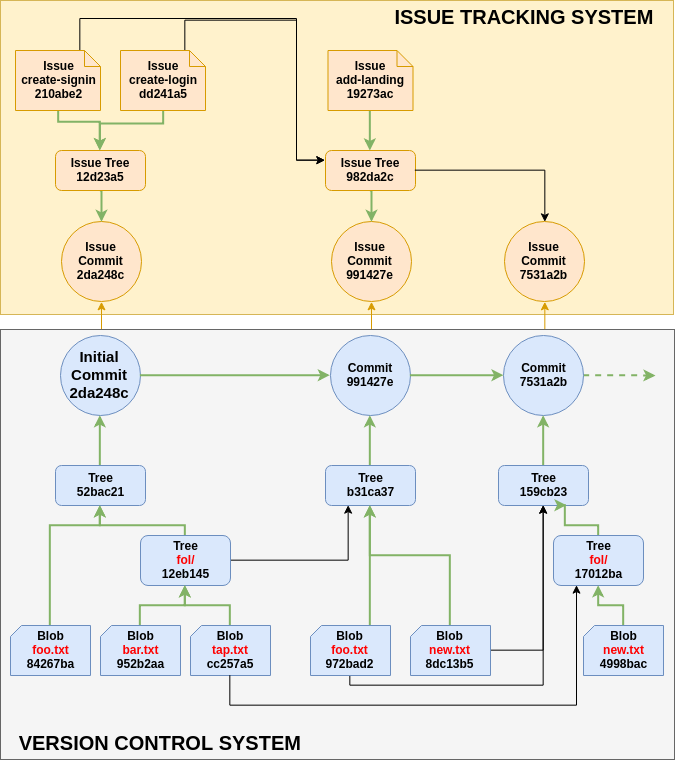
\includegraphics[width=10cm]{sciit-filesystem}
\end{figure}

Figure \ref{fig:sciit-filesystem} shows that every commit made in Git generates an issue commit that contains references to all the changes made to those issues. This therefore poses a change in the traditional management of issues. If an issue is changed by editing the issue data embedded in the soruce code as a comment then a new issue object is created and assigned to a new issue tree. Changes to the references of an issue object over time can now be associated with a change in the issue. The issue tracker also intuitively determines if issues are closed by removing references to an issue that has been deleted from the embedded comment.

% how it works in a distributed environment








\section{SCIIT's Distributed ITS}

%be explicit
As a result of embedding the ITS into a distributed VCS such as Git, the ITS is also a has a distributed structure. In Git the distributed structure involves the use of branching in which two different series of commits have deviated from one prior commit. Developers can spawn and work in new branches that are parallel to others. When complete they merge their changes with other branches. There are also remote Git repositories on servers where commits on branches are pushed and pulled to and from the local machine. 

Although branching and merging, pushing and pulling are the main mechanisims allowing Git to be distributed, they all are based on the same primative object, the commit. Since the ITS is based on this primative object, a branch commit will contain issue commits, issue trees and issues which may change over time. The utility of this design allows for the ITS to also be distributed.

The design concept gets compounded in merging senarios. In such events, developers can now be alerted by the VCS that there is a conflict with issues as source code content is compared. At this point developer team members can decide in their merges what changes should be made to the issue (edits or closure). Merge points are also represented as commit objects which the SCIIT system will again scan for embedded issues and update the issue references accordingly.

\begin{figure}[t]
\caption{Distributed Issue Tracking}
\label{fig:distributed-issue-tracking}
\centering
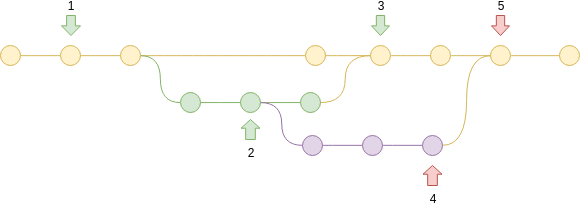
\includegraphics[width=15cm]{distributed-issue-tracking}
\end{figure}

Figure \ref{fig:distributed-issue-tracking} shows a practical example of the distributed ITS. At point 1 a new issue is added for the first time into the orange branch. Commits that follow this keep the reference the to issue created here until a user modifies the embedded issue information or removes it from the source code. When branching to green, issue 1 remains open in both branches. At point 2 another issue is created. Here there are two issues open on the green branch and one open on the orange. The purple branch inherits both issues from the green branch. At point 3, developers make the decision to merge issue 2 into the orange branch. At point 4, both issue 1 and 2 are closed by deleting the embedding from the source code. Here there are no issues on the purple branch. At point 5, developers decide that the work has actually been completed and resolves the merge conflict by deleting the two issue embeddings from the source code. This shows the distributred nature of issues.







\section{Software Architecture}

%% include more information on the architecture here
\begin{figure}[h!]
\caption{SCIIT Software Architecture}
\label{fig:sciit-software-arch}
\centering
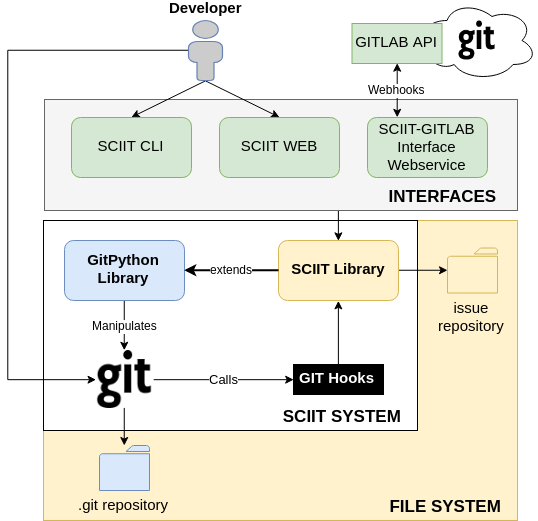
\includegraphics[width=10cm]{sciit-software-arch}
\end{figure}


Figure \ref{fig:sciit-software-arch} shows the software architecture of SCIIT. There are two seperate file system storage folders at the heart. One responsible solely for the VCS repository objects and the other for the ITS repository objects. The VCS information is accessed by the VCS control tool Git which in term can be manipulated by the GitPython Library. 

The SCIIT Library has direct access to the ITS repository and is responsible for managing all its objects stored within that context. This is its extended functionality. It aslo utilises objects, methods, and attributes of the GitPython Library in order to manipultate the VCS repository. This way the SCIIT Library can use information from both VCS and ITS to create, build and manage issues.

The Git hooks allow for the Git application to call on functions of the SCIIT Library when commit, merge, pull and checkout events take place. These hooks allow a level of automation in creating the ITS repository object such that developers need not concern themselves with explicitly maintaining the issue tracker. When these events take place the ITS is automatically managed.

Interfaces allow users to view issue tracking information stored in SCIIT. They provide direct access to the SCIIT Library that queries the ITS and VCS to build the information needed for the user. All combined these components make up the SCIIT system which allows for the manipulation of VCS and ITS objects.





\section{Summary}

This chapter shows the design of a Source Code Integrated Issue Tracker and how it embeds an ITS into a VCS. The benefit of this allows developers to focus on what they know and deal with the best which is source code. The next chapter will discuss how these designs were implemented to enable such a system to operate.









%%%%%%%%%%%%%%%%%%%%%%%%%%%%%%%%%%%%%%%%%%%%%%%%%%%%%%%%%%%%%%%%%%%
%%%%%%%%%%%%%%%%%%%%%%%%%%%%%%%%%%%%%%%%%%%%%%%%%%%%%%%%%%%%%%%%%%%
%%%%%%%%%%%%%%%%%%%%%%%%%%%%%%%%%%%%%%%%%%%%%%%%%%%%%%%%%%%%%%%%%%%
\chapter{Implementation}\label{implementation}

This chapter discusses the implementation of the design for providing mechanisms to interact with the integrated ITS. These are the use of Git Hooks for performing issue manipulation at certain Git events; the SCIIT Library which is an extension of the GitPython open source library to manipulate Git objects, Git commands and managing the Issue Repository; and the interfaces required to view and manage ITS information. The chapter continues by showing how issue tracking is performed and concludes outlining the challenges faced.

\section{Mechanisms}

\subsection{SCIIT Library - GitPython exteneded}

The first main mechanisms of SCIIT is the SCIIT Library. It is an extension of the GitPython open source library that enables the manipulation of the Git repository with new functionality to manage the Issue Repository. Funtionality in the GitPython library that are related directly to the Git repository are extended to provide the extra functionality needed for managing issues. Two programming library objects in particular are extended; the "Repository" object which allows for manipulating the Git repository and the "BaseObject" object allows for manipulating the raw Git objects (commits, trees, and blobs). Added to these were the ability to manipulate issues, issue trees, issue commits, and the issue repository.

% integrating git with sciit allows for the inference of many pieces of information required by issue trackers

\subsection{Git Hooks}

The second mechanism of SCIIT, Git Hooks, allows for the handling of issues based on Git events. In this project three hooks in particular are utilised; the post-commit, post-merge, and post-checkout. The post-commit hook comminicates with the SCIIT library in order to search for embeddings and create issues in the ITS for every commit made. This reduces friction since the programmer does not switch focus to the issue tracker for updating information. The post-merge hook is utilised during two Git events; merging and pulling. In order for SCIIT to be useful to teams, the issues that are created must be syncronised with all members of the team. When pulling commits from the remote repository, SCIIT will build issue objects that are missing. Similarly, during a merge, syncronisation ensures that no issues are missing. The post-checkout hook is similar to the merge in that it syncronises issue with commits. This is particularly implemented for the users that just fetch Git commits from the remote to checkout at a later stage.

\subsection{SCIIT Interfaces}

The last mechanism of SCIIT is its interface channels. There are three interface channels that provide three different services. 

\begin{figure}
\centering
  \caption{Tracker View in Terminal}
  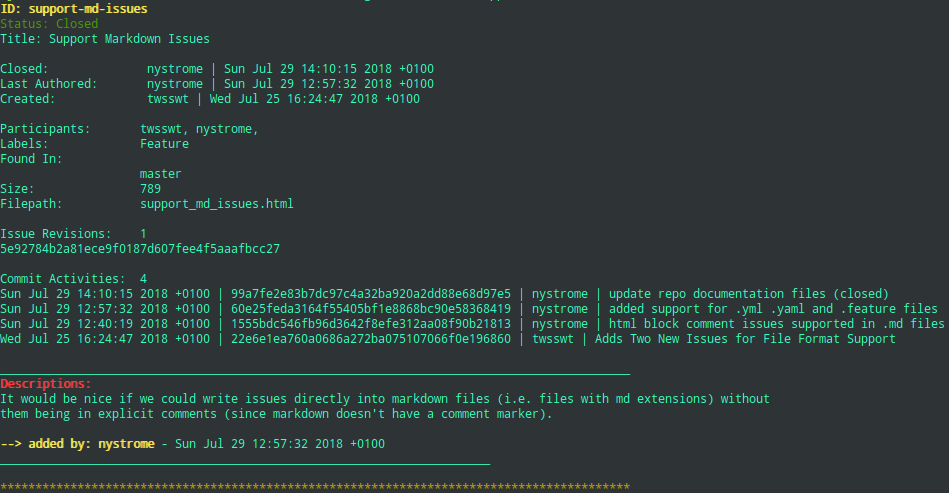
\includegraphics[width=15cm]{sciit-tracker-shot}
  \label{fig:sciit-tracker-shot}
\end{figure}


The first is a command line interface which does not allow for direct manipulation of issues but it allows for users to refresh the issue repository, view individual issues and view issue tracker. The initialisation commmand creates the issue repository and builds issues from past commits. This is essential since developers work on existing software projects. They can clone a project and build the ITS by grabbing all the embedded issues from commits. The tracker command allows developers to view details of issues. It shows the complex relationships between the ITS and VCS such as participants, creator, commits to the issue, and changes to the issue over time. This harnesses the power of ITS and VCS such that inferrence can be made between the two. Futher CLI commands and its uses can be found in Appendex B Figure \ref{fig:sciit-cheatsheet}. Figure \ref{fig:sciit-tracker-shot} shows an issue shown at the terminal.

The second is a web interface. This interface shows the issue tracker to the user by lauching a local web browser with all the issue tracking information loaded into html view. Users are not allowed to edit any of the information within this interface but it gives and easier display for users to view their issues, read through issue activity and view all other inferred data which performing developing tasks.

The thrid is an intermediate webservice that allows for the integration of GitLab issues with the SCIIT System. The main reason for having such an interface is that it allows for non developer members of a project such as coaches, team leads, production staff or contributors to create issues in GitLab that will create commits with embedded issues. This module was developed to show that SCIIT and its principles could be integrated with traditional ITS to engage non developer users. The webservice works by using GitLab Webhooks in conjuction with SCIIT on a webserver and the GitLab API as follows:

\begin{itemize}
  \item \textbf{Push Webhooks:} These hooks are triggered when developers push commits to the repository. A HTTP request is then sent to the SCIIT webservice interface. The interface then fetches the changes from the GitLab remote repository as a mirror repository and syncs the Git commits with the ITS issue references. Any new references that are made by these changes are then packaged and requests are made to the GitLab Issues API to create or edit those issues. Commit actitvities related to these changes are added to the GitLab issue as notes.
  \item \textbf{Issue Webhooks:} These hooks are triggered when someone creates or edits an issue in the GitLab web interface. A HTTP request is then sent to the SCIIT webservice interface. The interface then takes the issue title and issue description that was changed and makes changes to the relevant source code contents of the file that corresponds to the issue. If it has not been assigned to a file previously a new file is created to track the new issue. It then makes a request to the GitLab Commits API to create a new commit with the specified changes.
\end{itemize}

When this webservice is attached to the GitLab remote repository, it syncs GitLab issues, SCIIT issues and commits such that the developer need not be concerned that the issues they create or need to work on is not in the SCIIT system. A simple pull from the remote repository will bring in the related commits and refresh the issue tracker and its details.




\section{Issue Tracking}

The embedded ITS is no longer similar to the centralised ITS that are commonly found. In fact, the SCIIT Issue Tracker is decentralised and distributed and depends on the graph structure of branches and commits. It is accessed via an interface into the SCIIT Library and is built from a revision of the repository. A revision is a range of commits that is reachable from one commit to another. They can also be specified based on Git's intermediate references such as the HEAD or branch names and can span a path which may include all commits or those reachable from this branch.

As a distributed ITS, information about the issues are built by traversing the entire repository based on the revision. This is similar to Git operations such as the log where commits are walked through and commit inforation is displayed based on whether the commit is reachable from the revision specified. To build the issue tracker, commits and issue objects on this revision path are read and complex information between the ITS and the VCS are extracted. The following is a list of such information:

\begin{itemize}
    \item \textbf{Creator:} The creator and the date and time of creation can be identified by the first occurance of this embedded issue in the commit revision history. The author and time of that commit provides the exact information that reflects the creator of the issue.
    \item \textbf{Last Author:} The last author and the date and time of authoring can be identified as the last occurance of this embedded issue in the commit revision history. Similarly this provides the exact information required
    \item \textbf{Closed:} Again this information is extracted from the last commit mentioned that does not have the embedded issue. The person that has removed the embedded issue is the person that closed the issue.
    \item \textbf{Participants:} This is a list of persons that made commits that contained these issues. It adequately infers who has done work on the issues.
    \item \textbf{Branch Information:} This information is extracted showing the existance of issues on branches, and their status on branches. It can help the ITS user identify where issues are present and the status of their state.
    \item \textbf{Commit Activities:} This is a list that shows the date, commit message and commit author for every commit that has the issue present. It is one of the more powerful inferrence tools as it can show what work was done on issues over time and gives four main advantages. It represents real changes to the functionality and state of the software product as commits are made. It can contain a commit message the identifies precisely what progress has been made on an issue. It can tell us which developer contributed the change to the issue. It can give us the commit that contains the changes so that it can be reviewed.
\end{itemize}

The information inferred does not need to be explicitly entered into the issue tracker as it does in traditional ITS. This is the power of SCIIT where users need not be concerend about manually recording such information but it can be generated for them. See Appendix C Screenshots % Figure \ref{} and \ref{} which shows the issue tracker in the cli interface and on the web interface.



\section{Challenges}

Since the SCIIT system is first of its kind there are some challenges associated with its design and development. This section outlines the major design and development challenges.
% build time

The first major challenge concerns Git as a light weight system that invloves single threaded file access operations. When building the issue repository from past commits, SCIIT traverses each file object scans its contents to determine if an issue is persent or not. This is a time consuming process and can only be preformed in a single thread. If multiple threads, we will encounter I/O errors, especially since there is a high likelihood that the same file may be accessed or open in many threads. 

This limits the performance of SCITT to build issues from past commits on repositories that consist of a high number of commits such as the Linux Open Source Project or Tensorflow. The performace also suffers based on the commit/merge strategy that the developer teams are using since some strategies can have commits that contain a larger tree of file changes that other strategies. 

This also affects the performance of builing the issue tracker history as each object must be read in a single thread and added the the issue tracker history object. For very large repositories it can take some time for the issue tracker to be built which can reduce the productivity of the developer. The GitLab intergration webservice helps to reduce this problem, however, developer teams may user other remote hosting solutions for which integration services have not yet been created. This is the major challenge of the project and its design.

% communicating with webservice
The second major challenge concerns the use of GitLab API calls within the webservice interface. GitLab Webhooks are a part of the main functionality of the website. For example, utilising the GitLab Commits API triggers a Push Webhook. As such, during development special care needed to be taken to verify the dates of receiving GitLab webhooks with the internal webservice time. If a Webhook was triggered and came in within seconds of another they would be ignored as it would have originated from API calls within the webservice. In our webservice handling Issue Hooks generated requests for handling Push Hook and vice versa. If this was not carefully handled internally then the webservice would be in an infinate loop creating GitLab Issues and commit on the repository.


\section{Summary}

The implementation of the system ensures that developers are less burdened with the resposibility of maintaining an ITS as all the issues are now embedded into the VCS  commits. This should now reduce the friction between maintaining the issue tracker and developing code as the activities are now combined and automated.







%%%%%%%%%%%%%%%%%%%%%%%%%%%%%%%%%%%%%%%%%%%%%%%%%%%%%%%%%%%%%%%%%%%
\chapter{Evaluation}\label{evaluation}



This chapter begins by presenting the evaluation strategy. The remainder outlines SCIIT's merits and drawbacks as it relates to the reduction of friction between maintaining issue trackers and developing code, the impact on issue tracking practices, the impact on developing code using VCS, the feedback from test users and the robustness of the product as identified through software testing. 

\section{Evaluation Strategy}

SCIIT is evaluated by a process called Dogfooding. In progammer jargon, this is where developers use the product during development to determine useful features to include or to detremine fixs to unintended bugs before distribution. It provides high levels of feedback that are rapidly included in future releases. 

Alongside this, user testing is conducted with three students and the supervisor. Important points from feedback is discussed in the user feedback section. The software is also evaluated based on the stated objectives and the benefits and drawbacks of the design of the system.


\section{Reduction of Friction}

SCIIT provides a great contribution to reducing the friction between maintaining issue trackers and developing code. It allows for developers to be able to focus on the task of writing code and creating commits. In the background to this process SCIIT tracks revisions to issues and its references to commits. This way work can be done on an issue without need to manually update some ITS.

If the developer wishes to view the status of an issue they can call on the issue tracker from the command line interface or web interface and view the progress that has been made. Since it is built directly from the references of Git and Issue objects, the developer gets additional information. It is inferred and outlines other developers working on the issue, the issue creator, who closed the issue and what has been done. This information exists in this format for all memebers of the team without the need for it to be manually or explicitly defined.

When the need to change details of an issue arrises the developer does not need to login to another ITS or move their focus away from code. The embedded issue can be easy found using a text search in an IDE or through calling the tracker command from the CLI to be directed to the file containing the embedded issue. The developer can then make their updates to the metadata of the issue to include or remove the necessary details.

Additionally, since the issues are stored as embeddings within the source code, a clone of the repository will give a full copy of the issue history. This works well for new developers joining the team and does not require team leaders to setup two account for access to the codebase and access to issues. The issues are self conatined withing the code of the relevant project. This quality can also be useful in open source projects where the issues can be transferred during project forks. Finally, it saves the space and infrastructure required to maintain traditional ITS. 

By maintaining issues in this manner we can see that a significant step has been taken to reduce the friction between the two development activities of maintaining the ITS and VCS. Developer now need only concern themselves with pulling, and pushing code to the repository where the issue tracker will seemlessly build, track and maintain issues in the background.

This does not mean that developers are not resposible for looking at the embedded issues and performing the work required to implement them. However, it allows them to work in an environment with one point of contact. The design of SCIIT allows for developers to trod along writing code and to care for the issue tracking process. Additionally the issue tracker will now be up to date with the state of each revision of the source code.


\section{Impact on Issue Tracking Practices}

This section discusses the impact of SCIIT as a a new paradigm of an existing technology. SCIIT proposes some radical changes to the methods in which issue tracking is currently performed. In a traditional sense ITS are meant to be a centralised system containing all the knowledege objects in essentially one database. If we consider the distributed environment and that work is done in Git on branches, it could be difficult to capture all the information for all issues on all branches without conflicting data. 

Fortunately, Git also allows for the querying of revisions such that all commits on all branches are returned maintaining thier parental links. This allows us keep the valuable issue data for our project in a suitable archive. There is a limit to this however and circumstances where there is a potential for the loss of valuable data.

The product currently has no protection over the deletion of Git references. Indeed this is handled by Git itself which allows users to delete branches and to use functions such as rebasing that allows the mainpulation of commits and references. In cases such as these the issue commits may lose their references and there is a potential to loose those issues and its data forever, however few it may be. A permanement store may be required for the issues at some points of the development process to prevent such events.

Use of the integration webservice such as the provided gitlab webservice can provide a solution. Here information from the intermediate references between issues and commits are permanently stored in gitlab when a developer pushes to the remote repository. Additional to this the webservice also allows for non developers to interact with the SCIIT system where issues created in a traditional ITS creates commits with embedded issues in the VCS. This allows for developers to remain focused on creating code while not shutting out other organisational users of the ITS.

The integration of the traditional and SCIIT ITS provides just a method for more collaboration between various types of orgainisational users. This is an interrim approach to maintianing the levels of collaboration in the development of software. As SCIIT matures it can influnce both the development of ITS and VCS such that interrim services are no longer required.

\section{Impact on Developing Code Using VCS}

This section discusses the impact that SCIIT can have on developing code using VCS since it is the backbone component of the system. There are three development practices in VCS that are impacted by the integration of an ITS; pulling commits from remote collaboration repositories, creating detailed commit messages, influencing development workflows and branching strategy.

The integration of issues and code encourages developers to pull often so that they can have the latest changes made by other team members. Pulling often allows for the VCS and the ITS to be updated with the latest information. As X states, this is currently a software development best practice, as developers working in teams may contribute changes that affect the work of others. This form of collaboration and comminication keeps the developer teams aware of other work processes that are required to create high quality software products.

Commit messages in SCIIT are used as the basis for the log of work done on an issue. This encourages the use of detailed commit messages stating what has been changed added or fixed. Additionally, it also gives a higher quality status for the VCS as the messages used will provide a history of exactly what the commit contributed to the software product. Persons collaborating on this repository can now search the commit messages to find information on how to implement particular functionality, information on what was required to fix a bug, or imformation for educational purposes. This practice facilitates the ability for higher recall from the repository and benefits all members of the team.

Branching strategies are currently used to primarily manage the way in which software is merged. There are many theories for branching strategies and they help developers to follow a particular workflow when creating code so that their changes can be quickly integrated without significant problems. SCIIT is particularly designed to be useful to feature branching. This is where a developer creates a new branch of code from the main development brach in order to implement a new software feature. When work is done the feature is merged into the development branch or testing branch for integration testing and validation with the other code of the software product.

In SCIIT feature branching allows users to create their issues at the beginning of that branch and work on that issue till completion. Additionally, any branches from this feature branch can be considered to be related to this issue and also means that work done here contributes to the issue related to that feature. At the conclusion of the feature branch the issue can be closed and merged. SCIIT's influence on feature branching allows issues to remain in their own development line and is logically seperate from other types of work. This can be seen apparent in Figure \ref{fig:distributed-issue-tracking}

These areas are potentially affected by SCIIT and is a practical improvement to the workflow of developers. It encourages best practices and workflows that are industry standard. This however may not work well for all developer teams as some prefer to adopt their own style of developing. Futher use of the product in various different developer envirionments is required in order to assertain any wider impact on development and VCS practices that SCIIT may have.



\section{User Feedback}

This section describes the user experiences when using the SCIIT system. In particular it will cover its ease of use, how well it displays issues and its benefits and drawbacks.

\subsection{Ease of Use}

\subsection{Interfaces for Viewing Issues}

\subsection{Benefits and Drawbacks}


\section{Software Testing} % should I bother having a testing section

This section describes in detail the testing strategy that was used to verify the design and validity of SCIIT. The software is tested after the implementation of each desired feature this allows for regression testing with features already implemented. The test suite also utilises many mocks which mask the dependancies on other code in the system. Each test that requires access to the full Git repository is mocked out such that the test suite would finish running in sufficient time. Lastly, continuous integration (CI) practices are used to run the test suite as regression testing each time code is commited.

All modules of the software, except the intergration webservice, were throughly tested with unit and integration tests at the time of writing. However, the integration webservice tests are live to confirm its functionality. The test suite for the application is modular. The SCIIT Library, command line and web interfaces we all tested separately and a TestCase is made for each method within each module. Each TestCase contains atomic tests that verify the functionality of the method by checking valid and invalid senarios of operation, errors thrown, and boundary conditions. Currently, the test suite consists of 142 tests providing 98\% code coverage and verifies the stability of the application. 

During development CI practices were used to test regression of the application. Regression is where new fuctionality added breaks with well structured behaviour of methods. CI is where the entire test suite is run on every push to the remote repository. GitLab's CI is used since it offers the ability to send notificaitons on failed test cases. In these situations the applicaiton can be imediately updated to ensure that functionality is maintained.

This complete testing framework ensures that the SCIIT system developed conforms to the designs set out. This however does not mean that SCIIT is entirely free from bugs. More wide spread use of the system will uncover more bugs as users may try operations with the system that does not conform with its design intention. However, at its current release the system is stable for distribution and use.


\section{Summary}

The SCIIT system introduces changes into the way developers conduct software development practices since the ITS is embedded into the VCS. The softare practices are an emergent property of this design. Continued use and adoption will inform changes to development workflows as a result and the system will provide more insight and evaluation over time. However, at this stage, it is thoroughly tested and has a stable release for distribution.




%%%%%%%%%%%%%%%%%%%%%%%%%%%%%%%%%%%%%%%%%%%%%%%%%%%%%%%%%%%%%%%%%%%
\chapter{Conclusion}\label{conclusion}

This project shows that Issue Tracking Systems (ITS) can be successfully embedded into Version Control Systems (VCS) to reduce the friction between maintaining an issue tracker and developing code. The solution is a Source Control Integrated Issue Tracking (SCIIT) system that saves issues alongside commits in Git.

SCIIT benefits developers by allowing them to focus on the development process and create code. Issues are tracked by creating a small embedding in a block comment of the source code which are automatically tracked alongside the commits that developers create containing the issue. Through this developers are unburdened with the need to explicitly update an ITS.

The system provides a lightweight method for tracking issuses and potentially introduces new development workflows. Additionally, the system is a first of its kind and needs to mature before we can see additional benefits or unintended drawbacks from its use. It currently contains a feature set that allows it to replace traditional ITS but future work can be done to include features that enhance team collaboration.

\section{Future Work}

As discussed in literature, the ITS is a repository of knowledege that drives software development and learning. In order to continue in this vein, SCIIT must include other features that are persent in traditional ITS.

Adding the ability to comment on an issue is critical to communication. Comments on issues allow developers and various other stakeholders to discuss the effect of the issue on the software product or enterprise. For example, production and infrastucture teams may comment on an issue to give input on how it would affect the deployment of the software product after development.

Currently, SCIIT has no mechanisims for storing comments on issues. Creating such a mechanism will allow SCIIT to be much more valuable to developer teams and as such it is the next high priority feature item to be developed into this product. Once it is included it must again be tested for validity and be evaluated for its contribution to the software development process and its impact on VCS and ITS activities.

Commit activities is another area in which the system can be improved. Currently, commit activity is defined as any commit that contains the issue. This however is not totally accurate as teams may include issues into the software product as a guide of what work must be done. These issues may exist in the system however no work may be done on the issue until the appropriate time.

This leads to the need for context aware and programming language specific mechanisms that mark when work on an issue is actually started. Context aware mechanisms can be implemented through a marker on the issue to identify its state such as a future work, work in progress, or paused state. This way commit activity can be attributed to the accurate state of an issue which does not depend solely on its existance in the source code.

Programming language specific mechanisms can also be used to identify when work done on the source code relates to the issue. For example, issues present in a module or function block will have dependancies on other modules or functions. If the source code of the dependancy has changed then we can identify this as a commit activity on the issue.

These additional features will make the SCIIT system more robust and attune to the needs of both development teams and other software product stakeholders.


\appendix % first appendix
%%%%%%%%%%%%%%%%%%%%%%%%%%%%%%%%%%%%%%%%%%%%%%%%%%%%%%%%%%%%%%%%%%%
\chapter{CLI Cheatsheet}
\begin{figure}[h!]
\caption{SCIIT Command Line Interface Cheatsheet}
\label{fig:sciit-cheatsheet}
\centering
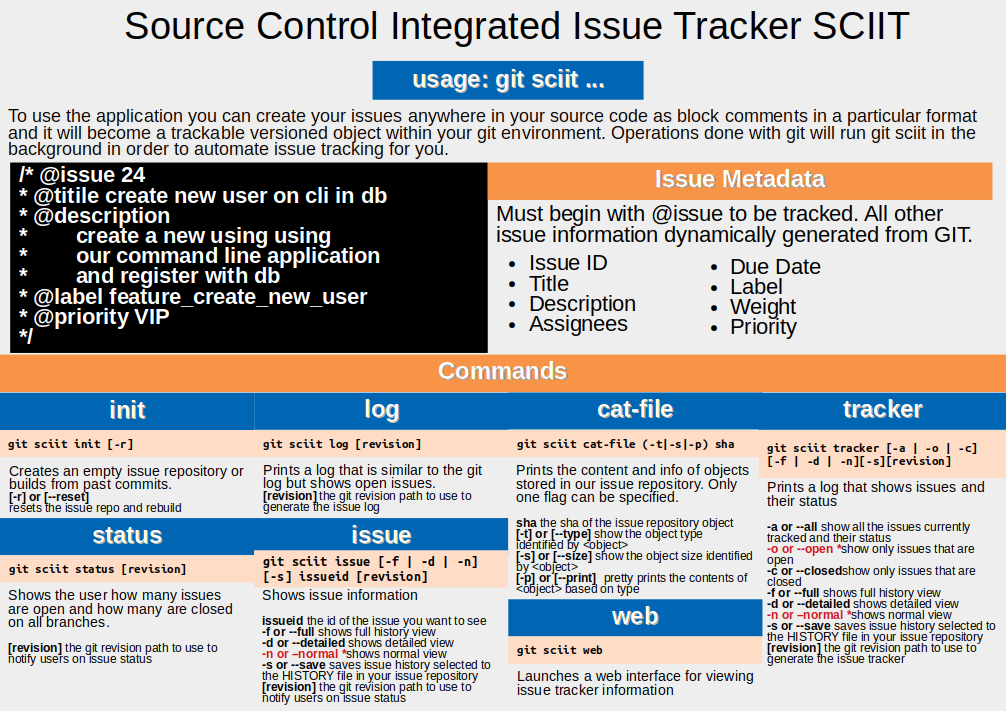
\includegraphics[width=16cm]{Cheatsheet}
\end{figure}

%consider making a diagram for the sciit webservice

%%%%%%%%%%%%%%%%%%%%%%%%%%%%%%%%%%%%%%%%%%%%%%%%%%%%%%%%%%%%%%%%%%%
% it is fine to change the bibliography style if you want
\bibliographystyle{acm}
\bibliography{mproj}
\end{document}
